\chapter{Ефекти впливу гамма--опромінення та ультразвукового навантаження на кремнієві структури метал-напівпровідник\label{Ch_GammaSD}}

\section{Cтруктури метал--напівпровідник на основі кремнію\label{MSSi}}

\begin{figure}[b]
\center
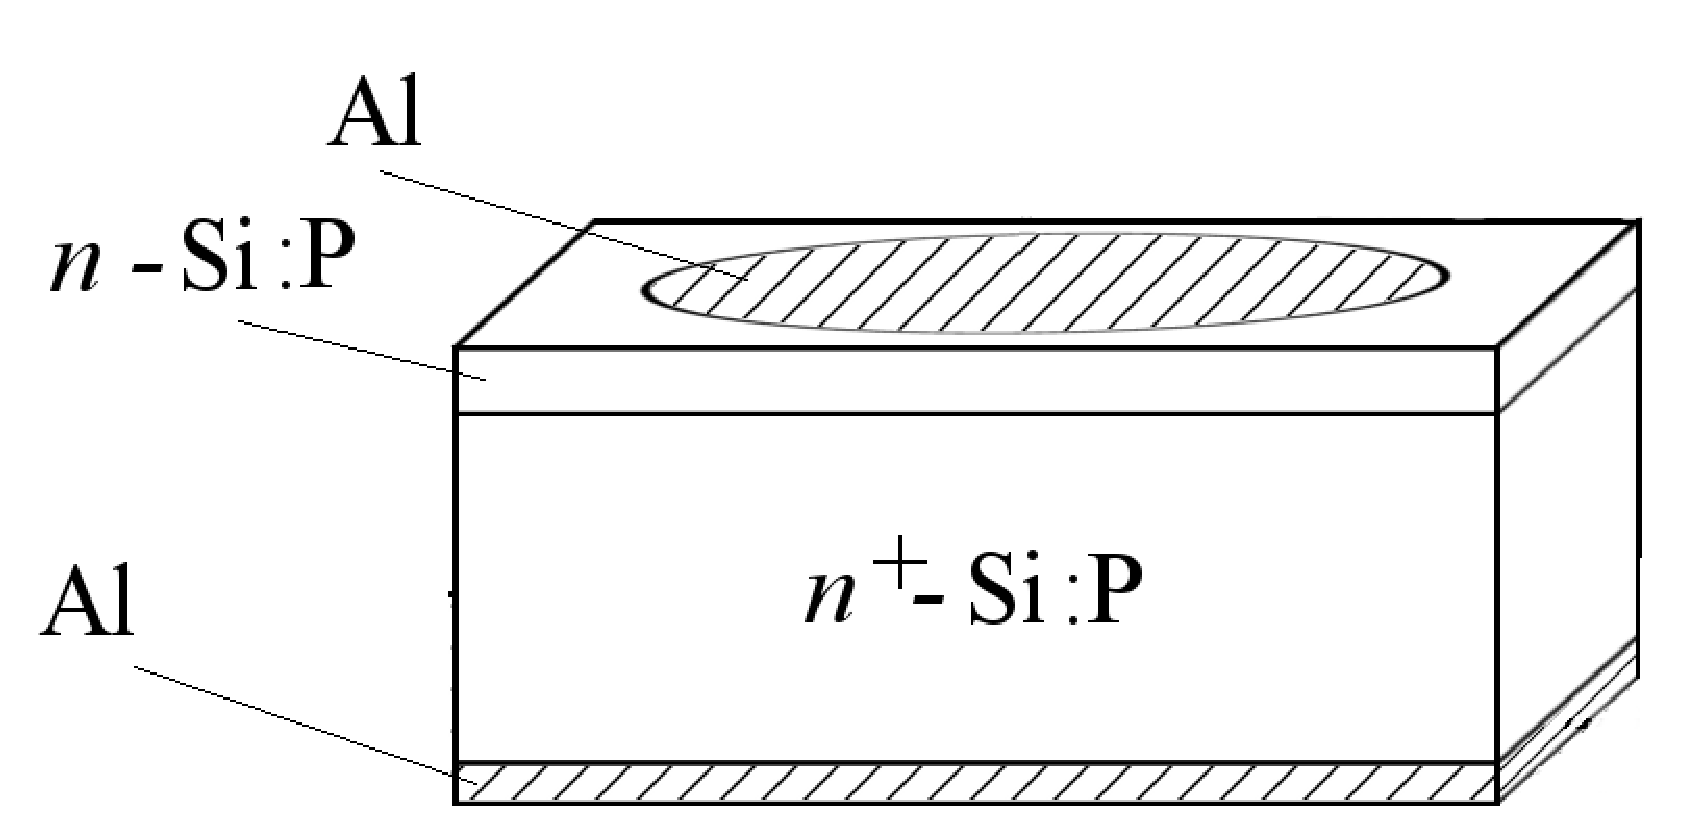
\includegraphics[width=0.65\textwidth]{MSSi}%
\caption{\label{figMSSi}
Структура зразків Mo$/n$--$n^+$--Si.
}
\end{figure}

В дослідженнях використовувалися структури МН (діоди Шотки (ДШ)), виготовлені на основі епітаксійної
структури $n$--$n^+$--Si.
Товщини епітаксійного шару та підкладки дорівнювали $0.2~\mu$м та $250~\mu$m, відповідно.
Епітаксійний шар був легований атомами фосфору, підкладка --- сурмою.
Для створення бар'єру на поверхню епітаксійного прошарку нанесено шар молібдену.
З протилежного боку структури нанесено прошарок алюмінію, який забезпечував наявність омічного контакту.
Схематичне зображення структур наведено на Рис.~\ref{figMSSi}.


В дисертації представлені результати, отримані з використанням кремнієвих ДШ двох типів,
які ідентичних за структурою, проте відрізняються концентраціями концентраціями носіїв заряду в епітаксійному шарі $N_d$ та
підкладці $N_s$, а також площею випрямляючого контакту $A$.
Для контролю рівня легування були виконані вимірювання вольт--фарадних характеристик (ВФХ) досліджуваних структур при кімнатній температурі ($T = 295$~К).
Параметри структур, а також їх позначення наведені в Таблиці~\ref{tabMSSi}.


\begin{table}
\caption{\label{tabMSSi}Параметри структур Mo$/n$--$n^+$--Si.
}
%\begin{tabular}{|c|c|c|c|}
\begin{tabularx}{\textwidth}{|>{\centering\arraybackslash}X|>{\centering\arraybackslash}X|>{\centering\arraybackslash}X|>{\centering\arraybackslash}X|>{\centering\arraybackslash}X|}
\hline
$N_d$, м$^{-3}$&$N_s$, м$^{-3}$&$A$, м$^2$&Позначення\\
\hline
$(1,1\div1,3)\cdot10^{23}$&$4,2\cdot10^{23}$&$3,14\cdot10^{-6}$&SSDA\\
\hline
$7,25\cdot10^{21}$&$4,2\cdot10^{22}$&$49\cdot10^{-6}$&SSDB\\
\hline
\end{tabularx}
\end{table}



\section*{Висновки до розділу \ref{Ch_GammaSD}}
\addcontentsline{toc}{section}{Висновки до розділу \ref{Ch_GammaSD}}
  \begin{enumerate}
     \item Проведено
  \end{enumerate}	
  
Основні результати даного розділу представлені в роботах \cite{Olikh:Rev,6CPFCS}.
